\section{Auswertung}
\label{sec:auswertung}
In diesem Versuch werden zwei Temperatur-Strom-Kurven mit unterschiedlichen Heizraten $b$ analysiert.
Messreihe A hat eine Heizrate von $b_{\text{A}}=\SI{2}{\kelvin\per\minute}$ und es wurde in dem Temperaturbereich
$T\in\left[\SI{213.1}{\kelvin},\SI{330.3}{\kelvin}\right]$ gemessen. Für Messreihe B beträgt die Heizrate
$b_{\text{B}}=\SI{1}{\kelvin\per\minute}$ und der vermessene Temperaturbereich ist $T\in\left[\SI{232.7}{\kelvin},\SI{289.6}{\kelvin}\right]$.
In beiden Fällen ist Kaliumbromid $\ce{KBr}$ der verwendete Kristall. Die Messdaten sind in Tabelle \ref{tab:Messdaten_roh}
abgebildet. 
\subsection{Bestimmung des Untergrundes}
Um den Untergrund zu bestimmen wird die Exponentialfunktion
\begin{equation}
    I_{\text{U}}(T) = C\cdot\exp\left(D\cdot  T\right)
\end{equation}
an die Messdaten vor und nach dem Peak gefittet.
Die Messdaten und die Fits sind in Abbildung \ref{fig:Untergrund_A} und \ref{fig:Untergrund_B} abgebildet.
\FloatBarrier
\begin{figure}
    \centering
    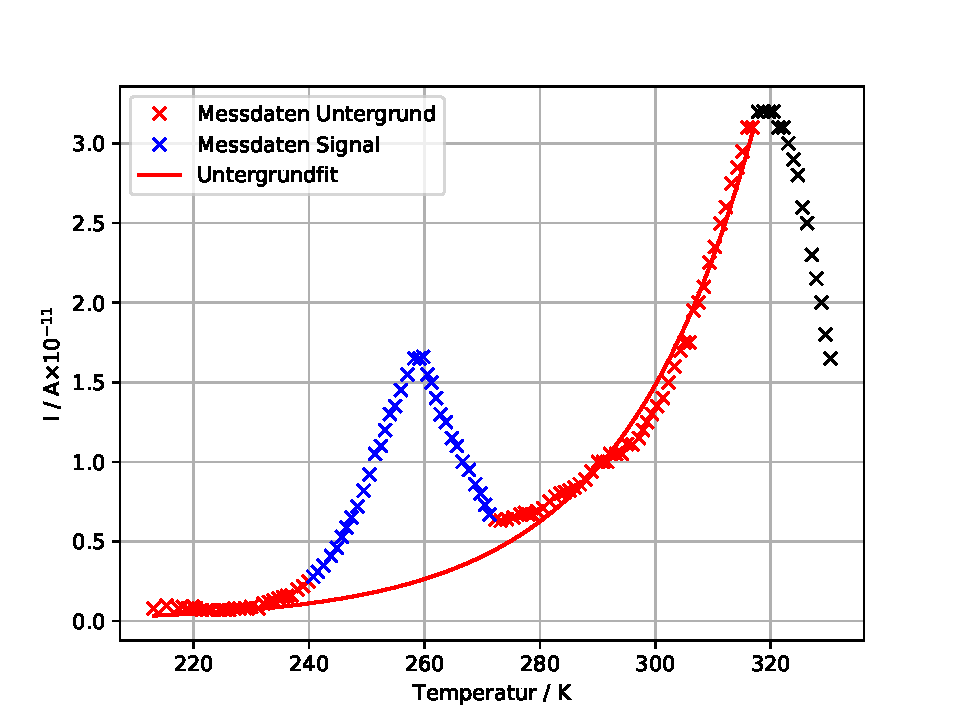
\includegraphics[width =\textwidth, keepaspectratio]{figure/Untergrund_A.pdf}
    \caption{Messdaten und Untergrundfit für Messreihe A, hierbei können die Messdaten nach dem zweiten Peak nicht für die 
    Bestimmung des untergrundes verwendet werden.}
    \label{fig:Untergrund_A}
\end{figure}
\begin{figure}
    \centering
    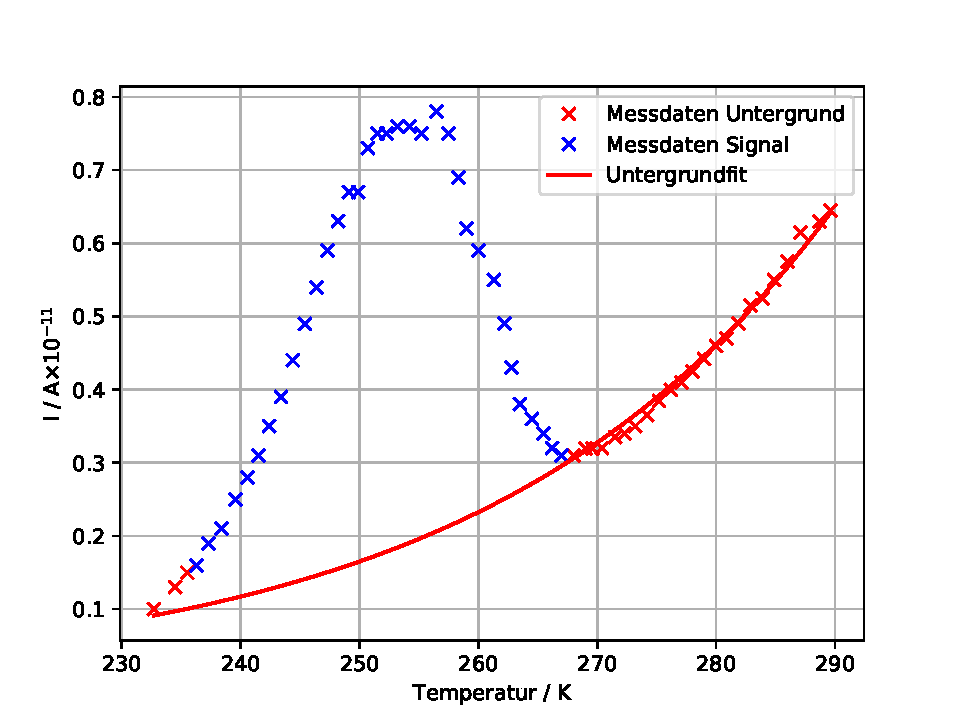
\includegraphics[width =\textwidth, keepaspectratio]{figure/Untergrundfit_B.pdf}
    \caption{Messdaten und Untergrundfit für Messreihe B.}
    \label{fig:Untergrund_B}
\end{figure}
\FloatBarrier
Die Fitparameter sind in der Tabelle \ref{tab:Fit_params_untergrund} aufgelistet.
\begin{table}
    \centering
    \caption{Fitparameter für die Untergrundfunktionen der beiden Messreihen.}
    \label{tab:Fit_params_untergrund}
    \begin{tabular}{c c c}
        \toprule
        Messreihe &$C\,/\,\SI{}{\ampere}$&$D\,/\,\SI{}{\per\kelvin}$\\
        \midrule
        A&$\num{3.5(9)e-6}$&$\num{0.0431(8)}$\\
        B&$\num{3.1(9)e-5}$&$\num{0.0343(10)}$\\
        \bottomrule
    \end{tabular}
\end{table}
\FloatBarrier
Um die Messreihe vom Untergrund zu bereinigen, werden von den gemessenen Stromwerten der Wert der Untergrundfunktion 
zu der dazugehörigen Temperatur subtrahiert. Die bereinigten Messwerte sind in Abbildung \ref{fig:Messdaten_bereinigt_A}
und \ref{fig:Messdaten_bereinigt_B} zu sehen.
\FloatBarrier
\begin{figure}
    \centering
    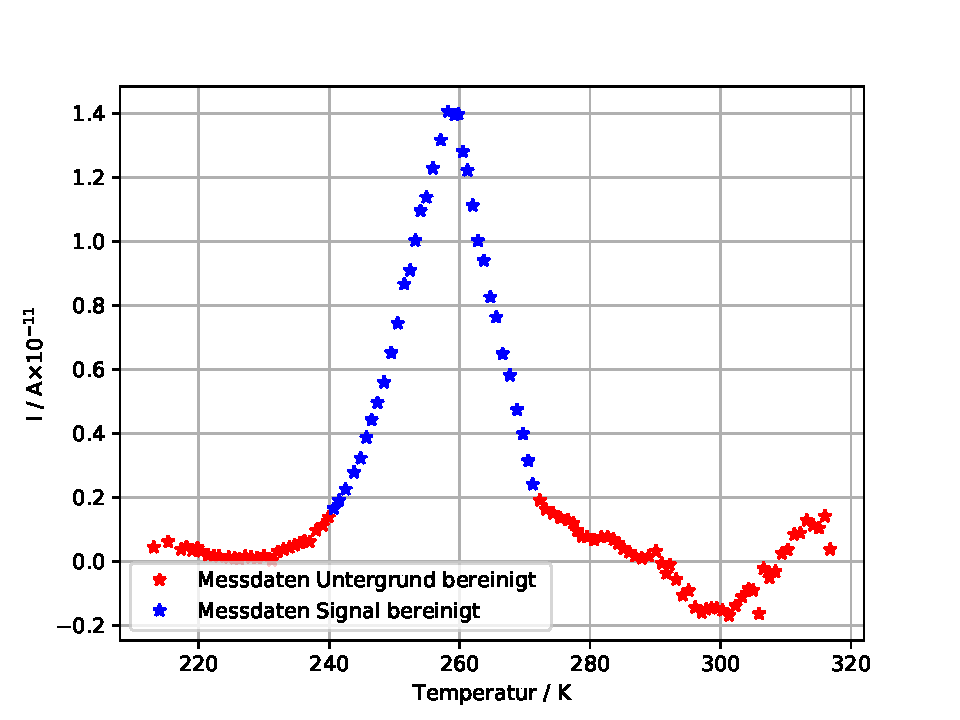
\includegraphics[width=\textwidth,keepaspectratio]{figure/Messdate_rein_A.pdf}
    \caption{Vom Untergrund bereinigte Messdaten der Messreihe A.}
    \label{fig:Messdaten_bereinigt_A}
\end{figure}
\begin{figure}
    \centering
    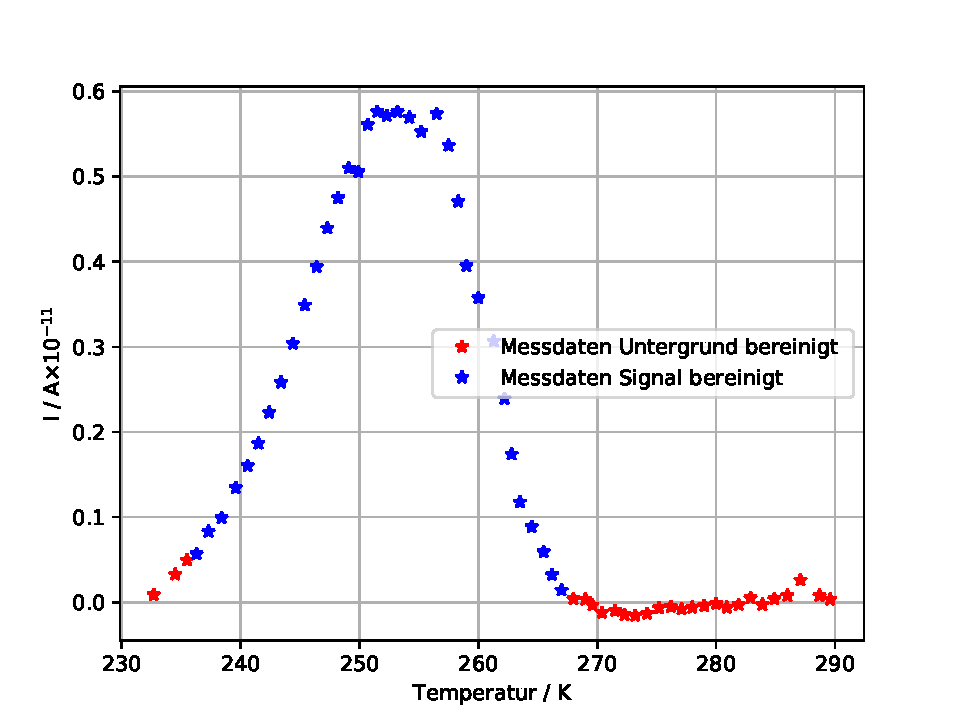
\includegraphics[width=\textwidth,keepaspectratio]{figure/Messdate_rein_B.pdf}
    \caption{Vom Untergrund bereinigte Messdaten der Messreihe B.}
    \label{fig:Messdaten_bereinigt_B}
\end{figure}
\FloatBarrier

\subsection{Niedertemperatur Approximation}
Um die Aktivierungsenergie $W$ zu ermittelt, wird die Gleichung \eqref{eq2} verwendet.
Dafür werden die bereinigten Messdaten der Messreihe A im Bereich $T_{\text{A}}\in \left[\SI{232.2}{\kelvin},\SI{253.2}{\kelvin}\right]$
und für Messreihe B im Bereich von $T_{\text{B}}\in \left[\SI{232.7}{\kelvin},\SI{250.7}{\kelvin}\right]$ logarithmiert und gegen $\frac{1}{T}$ aufgetragen.
Dazu wird eine lineare Ausgleichsgrade 
\begin{equation*}
    \text{ln}\left(I(T)\right) = \frac{-W}{k_{\text{{B}}}} \frac{1}{T} +\beta
\end{equation*}
angepasst. Hierbei ist der Fitparameter $W$ die Aktivierungsenergie des Kristalls.
Die logarithmiert Messdaten und die Ausgleichsgrade sind in den Abbildungen \ref{fig:Lin_fit_W_A} und \ref{fig:Lin_fit_W_B}
abgebildet.
\FloatBarrier
\begin{figure}
    \centering
    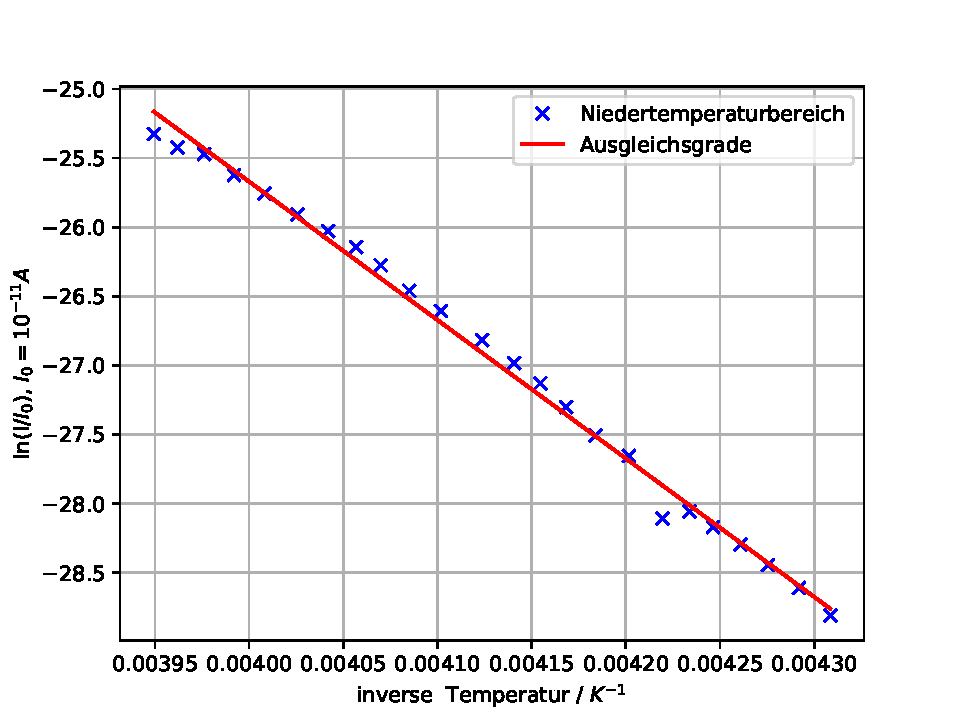
\includegraphics[width=\textwidth,keepaspectratio]{figure/LinFit_W_A.pdf}
    \caption{Messdaten und lineare Ausgleichsgrade für die Bestimmung der Aktivierungsenergie $W$ mit hilfe der Messreihe A.}
    \label{fig:Lin_fit_W_A}
\end{figure}
\begin{figure}
    \centering
    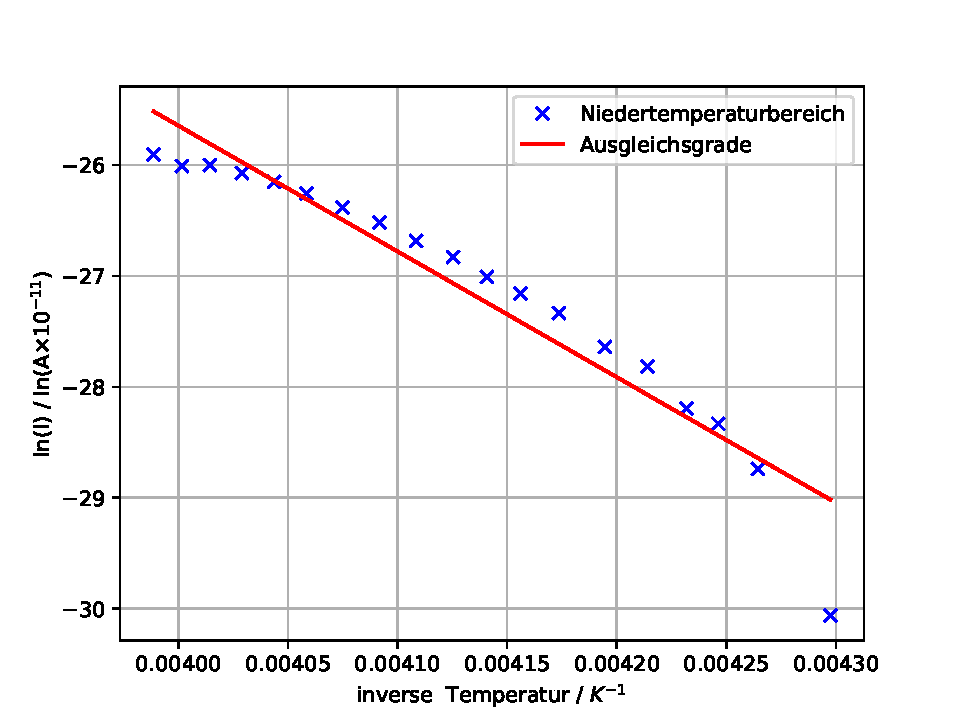
\includegraphics[width=\textwidth,keepaspectratio]{figure/LinFit_W_B.pdf}
    \caption{Messdaten und lineare Ausgleichsgrade für die Bestimmung der Aktivierungsenergie $W$ mit hilfe der Messreihe B.}
    \label{fig:Lin_fit_W_B}
\end{figure}
\FloatBarrier
Die Fitparameter sind in Tabelle \ref{tab:Niedertemperatur_approx_fit_params} abgebildet.
\begin{table}
    \centering
    \caption{Fitparameter der linearen Ausgleichsgraden der beiden Messreihen.}
    \label{tab:Niedertemperatur_approx_fit_params}
    \begin{tabular}{c c c c}
        \toprule
        Messreihe & $\beta \,/\, \ln(\SI{e-11}{\ampere})$&$W \,/\,\SI{}{\joule}$&$W \,/\,\SI{}{\milli\eV}$\\
        \midrule
        A&$\num{14.4(7)}$&$\num{1.383(23)e-19}$&$\num{863(14)}$\\
        B&$\num{19.7(34)}$&$\num{1.57(11)e-19}$&$\num{980(70)}$\\
        \bottomrule
    \end{tabular}
\end{table}
\subsection{Integrationsverfahren}
Bei dieser Methode wird die Aktivierungsenergie mithilfe der Gleichung \eqref{eq3}  bestimmt.
Das Integral aus Gleichung \eqref{eq3} wird numerisch mithilfe der Trapezregel bestimmt.
An die ermittelten Daten wird eine lineare Ausgleichsgrade der Form 
\begin{equation*}
    \ln{ \left( \frac{ \int_{T}^\infty j(T') \mathrm{d}T' }{ b j(T) \tau_{\text{0}} } \right) } = \frac{W}{k_{\text{{B}}}} \frac{1}{T} +\beta
\end{equation*}
angepasst. Der Fitparameter $W$ ist die Aktivierungsenergie.
Die Messdaten und die Fits sind in den Abbildungen \ref{fig:Integralverfahren_A} und \ref{fig:Integralverfahren_B} abgebildet.
\FloatBarrier
\begin{figure}
    \centering
    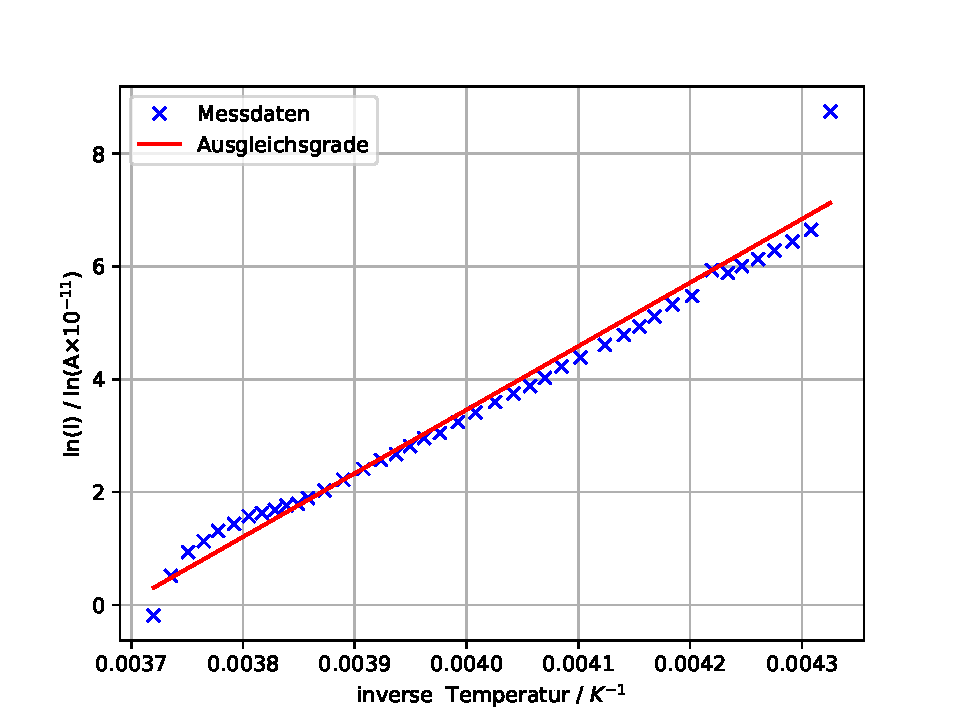
\includegraphics[width= \textwidth,keepaspectratio]{figure/Integralverfahren_A.pdf}
    \caption{Messdaten und lineare Ausgleichsgrade für die Bestimmung der Aktivierungsenergie mithilfe der Integrationsverfahrens für Messreihe A.}
    \label{fig:Integralverfahren_A}
\end{figure}
\begin{figure}
    \centering
    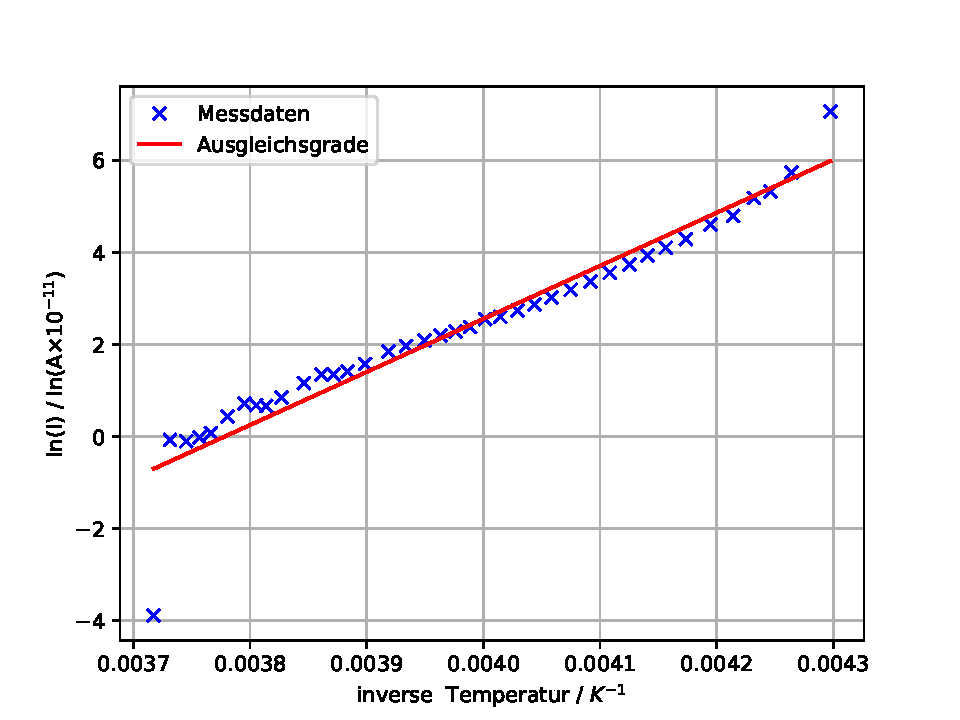
\includegraphics[width= \textwidth,keepaspectratio]{figure/Integralverfahren_B.pdf}
    \caption{Messdaten und lineare Ausgleichsgrade für die Bestimmung der Aktivierungsenergie mithilfe der Integrationsverfahrens für Messreihe B.}
    \label{fig:Integralverfahren_B}
\end{figure}
\FloatBarrier
Die Fitparameter der Ausgleichsgraden aus denn Abbildungen \ref{fig:Integralverfahren_A} und \ref{fig:Integralverfahren_B} sind 
in Tabelle \ref{tab:Fit_params_integtal} aufgelistet.
\begin{table}
    \centering
    \caption{Fitparameter der Ausgleichsgraden für die Bestimmung der Aktivierungsenergie mithilfe des Integrationsverfahrens.}
    \label{tab:Fit_params_integtal}
    \begin{tabular}{c c c c}
        \toprule
        Messreihe&$\beta \,/\, \ln(\SI{e-11}{\ampere})$&$W \,/\,\SI{}{\joule}$&$W \,/\,\SI{}{\milli\eV}$\\
        \midrule
        A&$\num{-41.6(14)}$&$\num{1.56(5)e-19}$&$\num{971(30)}$\\
        B&$\num{-43.6(23)}$&$\num{1.59(8)e-19}$&$\num{990(50)}$\\
        \bottomrule
    \end{tabular}
\end{table}
\subsection{Bestimmung der Relaxationszeit \texorpdfstring{$\tau_{0}$}{T1}}
Um die Relaxationszeit $\tau_{0}$ zu bestimmen wird die Funktion \eqref{eq:j_T} nach der Temperatur abgeleitet und 
die Temperatur bei Strommaximum eingesetzt und gleich Null gesetzt.
\begin{gather*}
    \left.\frac{\text{d}j(T)}{\text{d}T}\right|_{T_{\text{max}}}=0\\
    \implies \tau_0 = \frac{k_{\text{B}}T_{\text{max}}^2}{Wb}\exp{\left(-\frac{W}{k_{\text{B}}T_{\text{max}}}\right)}
\end{gather*}
$\tau_0$ wird mit den vorher bestimmten Ergebnissen der verschiedenen Methoden bestimmt.
Die verschiedenen $\tau_0$-Werte sind in Tabelle \ref{tab:tau_0} aufgelistet.
\FloatBarrier
\begin{table}
    \centering
    \caption{$\tau_0$-Werte der beiden Messreihen für die zwei Methoden der Bestimmung der Aktivierungsenergie.}
    \label{tab:tau_0}
    \begin{tabular}{c c c}
        \toprule
        Messreihe&$\tau_0\,/\,\SI{}{\second}$ (Approximationsverfahren)&$\tau_0\,/\,\SI{}{\second}$ (Integrationsverfahren)\\
        \midrule
        A&$\num{2.8(18)e-15}$&$\num{2.0(27)e-17}$\\
        B&$\num{8(30)e-18}$&$\num{4(9)e-18}$\\
        \bottomrule
    \end{tabular}
\end{table}
\FloatBarrier
Die Unsicherheiten sind sehr groß im Vergleich mit den bestimmten Werten, darauf wird in der Diskussion eingegangen.
Mit den $\tau_0$- und den $W$-Werten kann der Verlauf $\tau(T)$ dargestellt werden.
Diese sind in Abbildung \ref{fig:tau_verlauf_A} und \ref{fig:tau_verlauf_B} zu sehen.


















\section{Auswertung,Kevin}
Es werden in diesem Versuch zwei Messreihen mit unterschiedlicher Heizrate
$b$ durchgeführt. Zunächst müssen die Messwerte von Untergründen bereinigt
werden, auf die im Folgenden eingegangen wird.
Für die erste Messreihe -- im Folgenden mit dem Index A gekennzeichnet --
gilt $b_\text{A} = \SI{2}{\kelvin\per\minute}$, für die Zweite, mit B
gekennzeichnete Messreihe gilt $b_\text{B} = \SI{4}{\kelvin\per\minute}$.

Alle Fehler in dieser Auswertung werden -- wenn nicht anders beschrieben --
mittels Gaußscher Fehlerfortpflanzungen mit Hilfe des \texttt{python}-Paketes
\texttt{uncertainties} \cite{py-uncertainties} berechnet.

Zur Beschreibung des oben genannten Untergrundes wird bei Messreihe A eine
exponentielle Funktion $I_\text{bkg,A}(T)$ und bei Messreihe B eine lineare
Funktion
$I_\text{bkg,B}(T)$ von den Daten abgezogen. Die Variablen der Funktionen werden
durch Fit an einen Teil der Daten bestimmt, der in Abbildungen
\ref{fig:data-a} und \ref{fig:data-b} markiert ist.
Die Fitfunktionen haben die Gestalt
\begin{align*}
    I_\text{bkg,A}(T) &= A_1 e^{B_1 (T-T_0)} + C_1\,,\\
    I_\text{bkg,B}(T) &= A_2\cdot T + B_2\,.
\end{align*}
Das Resultat, sowie der Fit sind ebenfalls in oben genannter Abbildung
dargestellt und die entsprechenden Daten in den Tabellen \ref{tab:data1} und
\ref{tab:data2} aufgeführt.
Im weiteren Verlauf wird dabei jeweils ein offset $I_\text{off}$ von den Daten
abgezogen. Dieser beträgt für Datensatz A $I_\text{off} = \SI{1.46}{\pico\ampere}$
und für Datensatz B $I_\text{off} = \SI{8.1}{\pico\ampere}$.
Bei der ersten Messreihe ist auffällig, dass nur ein einzelner, flacher Peak
zu erkennen ist. Dies macht die spätere Auswertung extrem schwierig.
Aus diesem Grund werden die Ergebnisse der erste Messreihe im weiteren
Verlauf nicht betrachtet.

\subsection{Approximative Ausgleichsrechnung}
\label{subsec:approx}
Zunächst wird die in Abschnitt \ref{sub:berechnung_der_aktivierungsenergie_w_}
aufgeführte Gleichung \ref{eqn:approx} zur Bestimmung der Aktivierungsenergie
$W$ benutzt. Dabei wird diese mit einem nicht-linearen Fit in einem Bereich
$T$ zwischen \SIrange{250}{267}{\kelvin} an die Daten angepasst.
Das Ergebnis des Fits ist in Abbildung \ref{fig:fit_approx_set2} dargestellt.
Der Fit liefert von Messreihe A liefert



das entsprechende Ergebnis aus Messreihe B liefert



Die zugehörigen Fits sind in Abbildungen \ref{fig:fit_approx_set1}
und \ref{fig:fit_approx_set2} dargestellt.

\subsection{Ausgleichsrechnung mit Integration}
\label{subsec:integration}
Als zweite Methode zur Bestimmung der Aktivierungsenergie $W$ wird ein
linearer Fit der Form
\begin{equation*}
    F(T) = \alpha\cdot\frac{1}{T} + \beta
\end{equation*}
an die inversen Temperaturdaten $1/T$ durchgeführt.
Hierbei ist $F(T)$ wie in Gleichung \ref{eqn:integrate} definiert als
\begin{equation*}
    F(T) = \frac{\int_T^{T^\ast} i(T^\prime)\mathrm{d}T^\prime}{i(T)}\,.
\end{equation*}
Aus der Steigung $A$ lässt sich somit die Aktivierungsenergie $W$
berechnen durch
\begin{equation*}
    W = \alpha\cdot k_\text{B}\,.
\end{equation*}
Außerdem wird schließlich die Relaxationszeit $\tau_0$ aus der Temperatur
bei maximalem Strom $T_\text{max}$ bestimmt:
\begin{equation}
    \label{eqn:tau0}
    \tau_0 = \frac{k_\text{B}T_\text{max}^2}{Wb}
             \exp\!\left[-\frac{W}{k_\text{B}T_\text{max}} \right]
\end{equation}
Die Fits sind in Abbildungen \ref{fig:integrate_fit1} und \ref{fig:integrate_fit2}
dargestellt, sie liefern



für Datensatz A in einem Bereich $T \in [\SI{260}{\kelvin}, \SI{310}{\kelvin}]$ bei  und
für Datensatz B in einem Bereich $T \in [\SI{250}{\kelvin}, \SI{280}{\kelvin}]$ bei .
Die Fehler dieser Werte berücksichtigen jedoch keine systematischen Unsicherheiten
und werden daher stark unterschätzt. Darauf wird in der Diskussion weiter eingegangen.
\newpage
\section{Diskussion}
\label{sec:diskussion}
Alle hier durchgeführten Methoden zur Bestimmung der Aktivierungsenergie $W$
liefern Werte im erwarteten Bereich von einigen Millielektronvolt.
Die verschiedenen Messreihen liefern unterscheiden sich jedoch um einen Faktor
 (approximative Methode) beziehungsweise
 (integrierende Methode), was
auf systematische Fehler hindeutet und mit weiteren Messungen untersucht
werden muss.

Die mit Hilfe der integrierenden Methode bestimmten Werte der Relaxationszeit
$\tau_0$ sind schließlich nicht signifikant.
Die Fehler berücksichtigen nicht die starke Abhängigkeit von $\tau_0$ von der
Aktivierungsenergie $W$, die in Abbildung \ref{fig:_tau_test} dargestellt ist.
Bei einer Änderung von $W$ um einige \SI{100}{\milli\electronvolt} ändert
sich der Wert der Relaxationszeit bereits um etliche Größenordnungen.
Änderungen in diesem Bereich treten bereits auf, wenn der Wertebereich des Fits
leicht verändert wird und einige Meßpunkte mehr oder weniger betrachtet werden.
Die damit verbundenen Fehler machen eine Aussage über den wahren Wert von
$\tau_0$ unmöglich.
Die Unsicherheit $\Delta\tau_0$ sollte daher wesentlich zu größeren Werten hin
korrigiert werden.